\documentclass{BeamerTemplate}
\title{Module 10 - Régression linéaire simple}
\subtitle{STT-1000 Probabilités et statistique}

\date{Hiver 2023}

\usepackage{adjustbox}


\begin{document}
\AtBeginSection{\frame{\sectionpage}}

\begin{frame}

\titlepage

\end{frame}

\section{Introduction}

\begin{frame}[t]
 \frametitle{But d'une analyse de régression}

{\small

\alerter{Quels effets les variables explicatives $X_1,\, X_2,\, X_3,\,... $ ont-elles sur la variable réponse $Y$?}

\begin{itemize}\itemsep2mm
\item Quel est l'effet de la température sur la durée de vie  de la peinture sur l'asphalte?
\item Quel est l'effet d'un hiver très froid sur le niveau des réservoirs d'eau d'une ville en été?
\item Quels sont les effets des heures de sommeil, de sport et d'étude sur la note moyenne  d'un étudiant?
\end{itemize}
}
\end{frame}

\begin{frame}[t]{Objectifs plus précis}

{\small
Étudier les relations entre des variables en se basant sur des données}.

\begin{itemize}

\item \alerter{Prévision}: {\scriptsize {\it
Étant donné son âge, son poids, fumeur/non fumeur, combien
d'années un individu devrait-il survivre?}}

\item \alerter{Sélection de variables}: {\scriptsize {\it
Parmi la température, l'ensoleillement, la pluie reçue,
l'altitude, le trafic,  quelles variables ont une influence
significative sur la vitesse de l'orniérage des routes?}}

\item \alerter{Spécification de modèle}: {\scriptsize {\it
Comment la durée de vie de transformateurs électriques varie-t-elle
en fonction de leur grosseur?}}

\item \alerter{Estimation de paramètres}: {\scriptsize {\it
La luminosité en fonction de la distance des étoiles d'une certaine
galaxie est de la forme $L=K_1+K_2d+\sigma\varepsilon$, où $K_1$, $K_2$ et $\sigma$
sont des paramètres inconnus à être estimés à partir d'observations.}}
\end{itemize}

\end{frame}



%\subsection{Modèles de régression}

\begin{frame}[t]{Modélisation}

Exprimer la valeur de $Y$ \alerter{en fonction} des valeurs de $X_1,\ldots,X_{k}$:
$${\color{green}{Y}}=\alerter{f(}{\color{blue}{X_1,\ldots,X_{k}}}\alerter{)}+\text{fluctuation aléatoire}
$$

\hspace{1cm}
\begin{tikzpicture}[thick]
\draw [green, ->  ] (5.8,9) -- (4.2,8);
\draw [blue, ->    ] (8.2,9) -- (8,8) ;
\end{tikzpicture}

\begin{tabular}{ll}
{\color{green}{variable réponse}} & {\color{blue}{variables explicatives}}\\
{\color{green}{variable dépendante}} & {\color{blue}{variables indépendantes}}\\
{\color{green}{variable endogène}} & {\color{blue}{variables exogènes}}\\
{\color{green}{issue}} & {\color{blue}{facteurs}}\\
{\color{green}{ }} & {\color{blue}{covariables }}\\
\end{tabular}

\end{frame}

\begin{frame}[t]{Exemple d'un modèle à une variable}
%Soit $Y$, la masse d'un homme de 30 ans en kg et\\ soit $X$, sa grandeur en cm. On a que
%$$Y=f(X)+\mbox{fluctuation aléatoire}$$

$${\color{green}{Y}}\quad =\quad \alert{f(}{\color{blue}{X}}\alert{)}\quad +\quad \text{fluctuation aléatoire}
$$

\hspace{1cm}
\begin{tikzpicture}[thick]
\draw [green, ->  ] (5.6,9) -- (4.2,8);
\draw [blue, ->    ] (8.6,9) -- (7.8,8) ;
\draw [black, ->    ] (12,9) -- (12,8) ;
\end{tikzpicture}

\begin{tabular}{p{2cm}p{3cm}p{5cm}}
{\color{green}{masse d'un homme de 30 ans (kg)}} & {\color{blue}{taille de l'homme (cm) }}& deux hommes de 30 ans de même taille peuvent avoir une masse différente \\[2mm]
& {\color{blue}{(explique une partie de la masse) }}& (variation de la masse non expliquée par la taille)
\end{tabular}
\end{frame}


%\subsection{Régression linéaire}

\begin{frame}[t]{Modèle linéaire}
Un modèle de  régression \underline{linéaire}  représente $Y$ comme une \alerter{fonction linéaire des paramètres}:
$$
Y=\beta_0+\beta_1f_1(X_1)+\beta_2f_2(X_2)+\cdots+\beta_{k}f_{k}(X_{k})+E,
$$
\begin{itemize}
\item \alerter{$Y$}: variable réponse
\item \alerter{$X_1,\ldots,X_{k}$}: variables explicatives
\item \alerter{$f_1,\ldots,f_{k}$}: transformations connues des variables explicatives
\item \alerter{$\beta_0,\ldots,\beta_{k}$}: paramètres de valeur inconnue à estimer à l'aide d'observations.
\item \alerter{$E$}: erreur aléatoire
\end{itemize}
\end{frame}

\section[Rég. lin. simple]{La régression linéaire simple}


\begin{frame}[t]{Modèle de régression linéaire \underline{simple} (RLS)}

\alerter{Une seule variable explicative $X$}, liée à $Y$ par une droite.

\medskip
%Utile pour modéliser la relation entre $X$ et $Y$ lorsqu'un
$n$ paires d'observations indépendantes $(X_1,Y_1),\ldots,(X_n,Y_n)$, réparties autour d'une droite imaginaire.\\

\vspace{5mm}

\begin{minipage}[b]{5cm}{
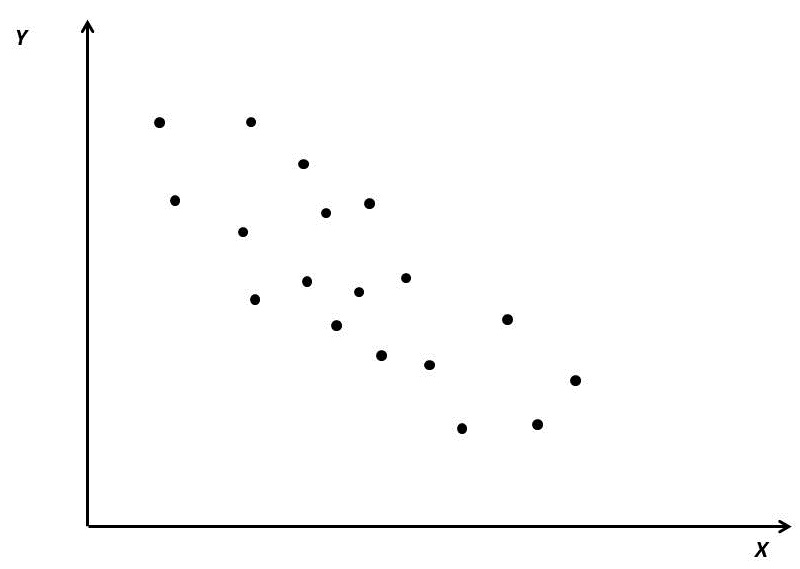
\includegraphics[width=5cm]{RLS1a.jpg}
}
\end{minipage}
\begin{minipage}[b]{5cm}{
${\color{green}{Y_i}}\quad=\quad{\color{blue}{\beta_0+\beta_1X_i}}\quad+\quad E_i$\\ \hspace{2cm} $(i=1,\ldots,n)$

\vspace{0.5cm}
\underline{Postulats}:\\
\alerter{$Y_i\sim N(\beta_0+\beta_1X_i,\sigma^2)$ indép.}

équivalent à

\alerter{$E_i\sim N(0,\sigma^2)$ indép.}
\vspace{0.5cm}

}
\end{minipage}
\end{frame}


\begin{frame}[t]{Les postulats du modèle}

{\small
Conditions d'application à vérifier avant d'interpréter les intervalles de confiance et les tests d'hypothèses à venir:
\begin{itemize}\itemsep2mm
\item[P1] {\bf  linéarité:} la moyenne de $Y_i$ est linéaire par rapport à $X_i$;\\
    {\color{gray}{ $E(Y_i)=\beta_0+\beta_1X_i \hspace{1cm} \Rightarrow E(E_i)=0$ }}
\item[P2] {\bf homoscédasticité:}  la variance de $Y_i$ autour de la droite est homogène (elle ne dépend pas de $X_i$);\\
    {\color{gray}{$V(Y_i)=\sigma^2 \hspace{2cm}\Rightarrow V(E_i)=\sigma^2$}}
\item[P3]  {\bf indépendance:}  les observations sont indépendantes;\\
    {\color{gray}{ $Y_i$indépendants \hspace{1.1cm} $\Rightarrow$  $E_i$ indépendants}}
\item[P4]  {\bf  normalité:} les $Y_i$ sont de loi normale autour de la droite.\\
    {\color{gray}{ \hspace{3.5cm} $\Rightarrow$ les $E_i$ sont de loi normale autour de 0}}
\end{itemize}
}
\end{frame}


\begin{frame}[t]{Éléments du modèle de RLS}
\centerline{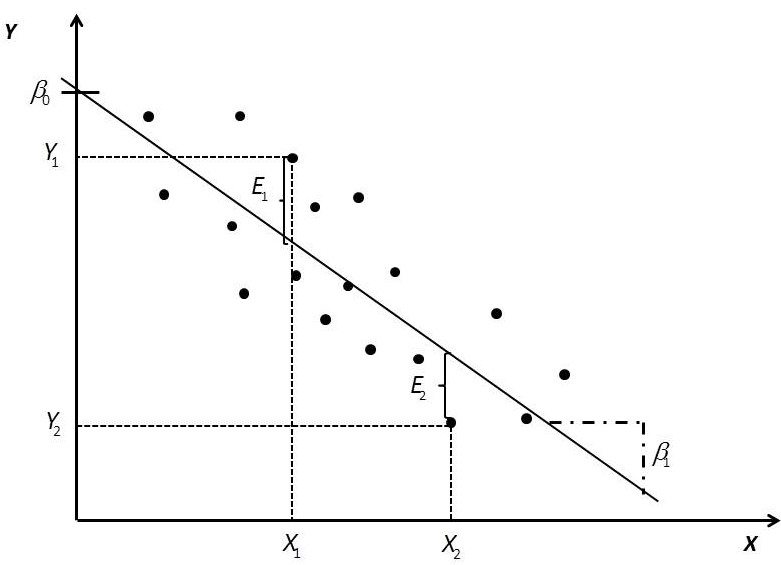
\includegraphics[height=6cm]{RLS1b.jpg}}
\end{frame}

\begin{frame}[t]{Interprétation des paramètres $\beta_0$ et $\beta_1$}

Si le postulat de linéarité (P1) est vrai:
\begin{itemize}\itemsep2mm
\item<1-> {\color{blue}{$\beta_1$}}: \alerter{Si on augmente $X$ d'une unité, alors la valeur moyenne de $Y$ augmente de $\beta_1$
unités}.\\
$\bullet$  $\beta_1>0$:  grands $X$  associés aux grands $Y$ et vice-versa (corrélation positive entre les variables). \\
$\bullet$  $\beta_1<0$:  petits  $X$ associés aux grands  $Y$.
\item<2-> {\color{blue}{$\beta_0$}}:  \alerter{la valeur moyenne de $Y$ quand $X=0$}.\\
$\bullet$ Si $X=0$ est peu plausible en pratique, $\beta_0$ peut prendre une valeur farfelue, mais le modèle de régression linéaire simple reste adéquat pour les valeurs de $X$ près de celles observées.
\end{itemize}

\end{frame}

\begin{frame}[t]{Extrapolation dangereuse!}

{\small
%Soit $Y_i$ le rendement d'un procédé chimique et $X_i$ la concentration d'un certain catalyseur lors de la $i$-ème répétition d'une expérience, $i=1,\ldots,10$.
On ignore la forme de la relation entre $X$ et $Y$ à l'extérieur de l'intervalle observé.
}

\centerline{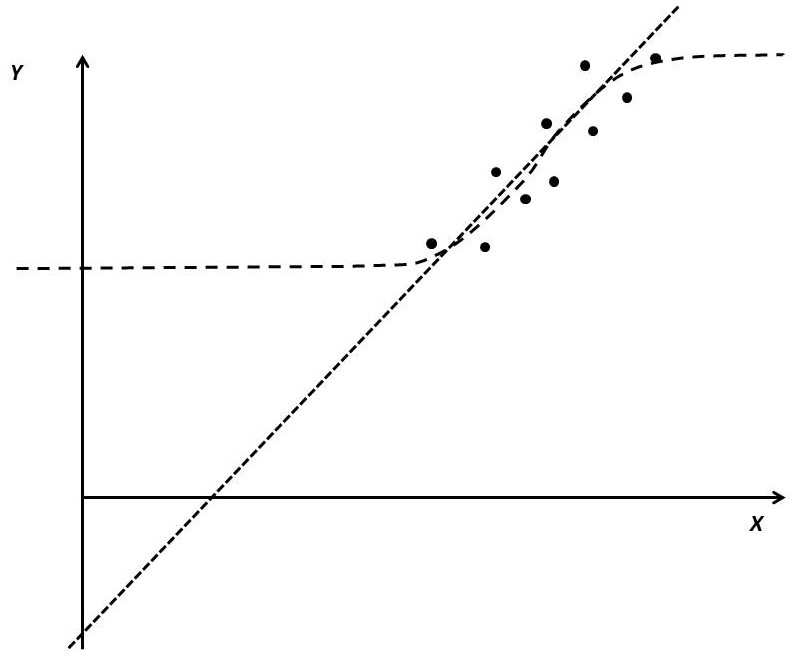
\includegraphics[height=5.25cm]{extrapol.jpg}}
\end{frame}


\begin{frame}[t]{Estimation des paramètres  $\beta_0$ et $\beta_1$}

{\small
%En pratique, on observe $(X_1,Y_n),\ldots,(X_n,Y_n)$ mais on n'observe pas la vraie droite, c.-à-d.,
$\beta_0$ et $\beta_1$ : paramètres de valeurs inconnues.\\[1mm]
$\hat{\beta}_0$ et $\hat{\beta}_1$ : estimateurs des paramètres, obtenus en \alerter{minimisant la partie inexpliquée de $Y$} (la fluctuation aléatoire):

\medskip


$$
SS_E\quad=\quad\sum_{i=1}^ne_i^2\quad=\quad\sum_{i=1}^n(Y_i-\hat{Y}_i)^2\quad=\quad\sum_{i=1}^n(Y_i-\hat{\beta}_0-\hat{\beta}_1X_i)^2,
$$
où

\begin{itemize}
\item \alerter{$\hat{Y}_i$ }$=\hat{\beta}_0+\hat{\beta}_1X_i$ est la $i^e$ \alerter{valeur ajustée}, ou \alerter{valeur prédite} \\(la partie de $Y_i$ expliquée par le modèle)
\item \alerter{$e_i$}$=Y_i-\hat{Y}_i$ est le $i^e$ \alerter{ résidu} \\(la partie de $Y_i$ inexpliquée par le modèle).
\end{itemize}
}
\end{frame}
\begin{frame}[t]{Problème de minimisation}
En annulant les dérivées de $SS_E$ par rapport à $\hat\beta_0$ et $\hat\beta_1$, on obtient


$$\begin{array}{|ll|}\hline &\\[-2mm]

\hat{\beta}_1&
=\dfrac{S_{XY}}{S_{XX}}\\[6mm]
\hat{\beta}_0&=\overline{Y}-\hat{\beta}_1\overline{X}\\[3mm]\hline
%\end{align*}
\end{array}$$

où\\

{\small
$S_{XX}=\sum\limits_{i=1}^n(X_i-\overline{X})^2\qquad = \qquad (n-1)\,s_X^2\quad = \quad\sum\limits_{i=1}^nX_i^2-n\overline{X}^2$

\bigskip
$S_{XY}=\sum\limits_{i=1}^n(X_i-\overline{X})(Y_i-\overline{Y})=\;\sum\limits_{i=1}^n(X_i-\overline{X})Y_i\;\;=\;\;
\sum\limits_{i=1}^nX_iY_i-n\overline{X}\overline{Y}.$
}
\end{frame}

\begin{frame}[fragile]
\frametitle{Exemple 1: Absorption d'oxygène chez\\ 24 hommes qui courent 3,2 km}

\begin{minipage}[b]{4.5cm}
{\tiny
\begin{verbatim}
      VOLUME MAX.  TEMPS EN
SUJET   D'O2 (Y)  SECONDES (X)
   1       42.33      918
   2       53.10      805
   3       42.08      892
   4       50.06      962
   5       42.45      968
   6       42.46      907
   7       47.82      770
   8       49.92      743
   9       36.23     1045
  10       49.66      810
  11       41.49      927
  12       46.17      813
  13       48.18      858
  14       43.21      860
  15       51.81      760
  16       53.28      747
  17       53.29      743
  18       47.18      803
  19       56.91      683
  20       47.80      844
  21       48.65      755
  22       53.69      700
  23       60.62      748
  24       56.73      775
\end{verbatim}

\vspace{1cm}
}
\end{minipage}
\begin{minipage}[b]{6cm}{
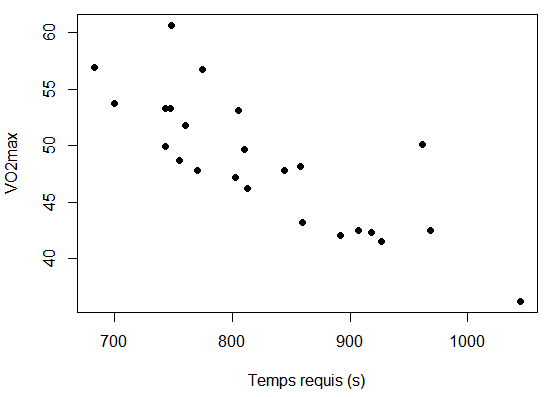
\includegraphics[width=5.9cm]{Ex9_4-R1.png}
}\end{minipage}
\end{frame}


\begin{frame}[t]{Exemple 1: Estimation des paramètres}

{\small %Avec {\it R Commander} ... ou à la main: on a que
On a effectué les calculs suivants:
\medskip

$\begin{array}{lll}
\overline x = 826,5\qquad\qquad & s_X^2 = 8593,8\qquad\qquad & \sum\limits_{i=1}^{24}x_iy_i=952\,885\\[3mm]
\overline y = 48,55& s_Y^2 = 34,1&  \\

\end{array} $

\medskip
Quelle est l'équation de la droite de régression estimée?}

$\hat\beta_1=\dfrac{S_{XY}}{S_{XX}}$

\vspace{7mm}

$\hat\beta_0=\overline{Y}-\hat{\beta}_1\overline{X}$

\vspace{7mm}

$\hat Y=\hat\beta_0+\hat\beta_1\,X$
\end{frame}


\begin{frame}[t]%{Événements mutuellement exclusifs}

\centerline{\LARGE \bf \alert{QUIZ !}}
\begin{itemize}\itemsep1cm
\item Jacques a couru les 3,2 km en 10 secondes de plus que Marc, mais ils n'ont pas mesuré leur $VO_2max$. Quelle différence de $VO_2max$ le modèle ajusté prédit-il entre les deux hommes?
\item Vrai ou Faux: on peut dire que les hommes qui courent le 3,2 km en 0 seconde ont un $VO_2max$ moyen de 90,7.

\vspace{1cm}
\end{itemize}

\end{frame}

\begin{frame}[t]{Relation non significative entre $Y$ et $X$}
Si le postulat de linéarité est respecté, alors \alerter{une pente nulle pour la droite de régression ($\beta_1=0$) signifie qu'il n'y pas d'association entre les variables $Y$ et $X$}.
\medskip

Dans ce cas,  la loi de $Y$ ne change pas avec la valeur de $X$ (la valeur moyenne de $Y$ est égale à
$\beta_0$ peu importe la valeur de $X$.)

%En effet, dans ce cas on a que $E(Y|X)=\beta_0+\beta_1X=\beta_0+0X=\beta_0$, et donc
\centerline{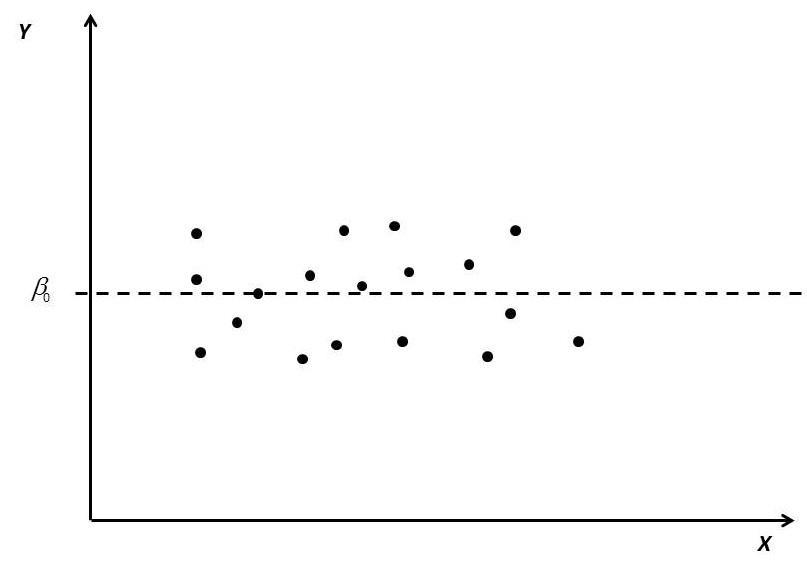
\includegraphics[height=4.5cm]{beta1nul.jpg}}

\end{frame}


\begin{frame}[t]{Tests sur la significativité de la relation linéaire}
Il existe deux approches équivalentes pour tester:
$$
H_0:~\beta_1=0\text{\ \ \ \ vs\ \ \ \ }H_1:~\beta_1\neq0.
$$


\vspace{0.5cm}

Il s'agit du test $F$, basé sur l'analyse de la variance et du test $t$ sur $\beta_1$.

\alerter{Dans ce cours, nous ne verrons que le test $t$.}
\end{frame}



\begin{frame}[t]{Approche basée sur la loi $t$}

{\small
On peut utiliser le fait que
\begin{align*}
\hat{\beta}_1&=\frac{S_{XY}}{S_{XX}}=\frac{\sum_{i=1}^n(X_i-\overline{X})Y_i}{\sum_{i=1}^n(X_i-\overline{X})^2}
=\sum_{i=1}^n\left[\frac{(X_i-\overline{X})}{\sum_{i=1}^n(X_i-\overline{X})^2}\right]Y_i
\end{align*}
est une combinaison linéaire des $Y_i\Rightarrow$
$$
\hat{\beta}_1\sim N\left(\beta_1,\frac{\sigma^2}{S_{XX}}\right)\Leftrightarrow
\frac{\hat{\beta}_1-\beta_1}{\sqrt{\frac{\sigma^2}{S_{XX}}}}\sim N(0,1)
$$

Par contre, nous ne connaissons pas $\sigma^2$. Il faut donc l'estimer. 



}
\end{frame}

\begin{frame}{}
Comme $\sigma^2$ est la variance des erreurs du modèle $E_i=Y_i=\beta_0-\beta_1 X_i$ que nous estimons par $e_i=y_i=\hat{\beta_0}-\hat{\beta_1} x_i$, nous utiliserons

$$\hat{\sigma}^2=MS_E= \frac{SS_E}{n-2}.$$
Nous en déduisons donc
\alerter{$$
T_0=\frac{\hat{\beta}_1-\beta_1}{\sqrt{\frac{MS_E}{S_{XX}}}}\sim t_{n-2}.
$$}
\end{frame}
\section{Intervalles de confiance et de prédiction}

\begin{frame}[t]{Estimateurs de $\beta_0$ et $\beta_1$}

\centerline{$Y_i=\beta_0+\beta_1X_i+E_i,\ \ \quad E_i\;\sim\;N(0,\sigma^2)$}

\bigskip

{\small
%Les vraies valeurs de $\beta_0$ et $\beta_1$ sont inconnues, et estimées en minimisant $SS_E$:

{\renewcommand{\arraystretch}{2}
$\begin{array}{c|c|c}
\text{Paramètre}&\text{Pente}&\text{Ordonnée à l'origine}\\\hline
\text{Estimateur}&\hat{\beta}_1%=\frac{\sum_{i=1}^n(X_i-\overline{X})Y_i}{\sum_{i=1}^n(X_i-\overline{X})^2}
=\dfrac{S_{XY}}{S_{XX}}%=\dfrac{\sum_{i=1}^n(X_i-\overline{X})Y_i}{\sum_{i=1}^n(X_i-\overline{X})^2}
&\hat{\beta}_0=\overline{Y}-\hat{\beta}_1\overline{X}\\\hline
\text{Espérance}&\beta_1&\beta_0\\\hline
\text{Variance}&\dfrac{\sigma^2}{S_{XX}}&\dfrac{\sigma^2}{n}+\dfrac{\sigma^2\,\overline X^2}{S_{XX}}\\[2mm]\hline
\text{Stat. inférence}& \dfrac{\hat{\beta}_1-\beta_1}{\sqrt{\dfrac{MS_E}{S_{XX}}}}\sim t_{n-2}& \dfrac{\hat{\beta}_0-\beta_0}{\sqrt{MS_E\left(\frac{1}{n}+\frac{\overline{X}^2}{S_{XX}}\right)}}\sim t_{n-2}
\end{array}$
}

}
\end{frame}

\begin{frame}[t]{Intervalle de confiance pour $\beta_1$}

On a que
$$P\left(-t_{\alpha/2;n-2}\le\frac{\hat{\beta}_1-\beta_1}{\sqrt{MS_E/S_{XX}}}\le t_{\alpha/2;n-2}\right)=1-\alpha.$$

En isolant $\beta_1$ au centre, on obtient l'intervalle de confiance de niveau $1-\alpha$  suivant pour
$\beta_1$:
{\color{blue}{$$
\hat{\beta}_1\pm t_{\alpha/2;n-2}\sqrt{\frac{MS_E}{S_{XX}}}.
$$}}
\end{frame}


\begin{frame}[t]{Intervalle de confiance pour $\beta_0$}

$\hat{\beta}_0$ est aussi une combinaison linéaire des $Y_i$, donc
$$
\frac{\hat{\beta}_0-\beta_0}{\sqrt{MS_E\left(\frac{1}{n}+\frac{\overline{X}^2}{S_{XX}}\right)}}\sim t_{n-2}.
$$

On obtient l'intervalle de confiance de niveau $1-\alpha$   pour
$\beta_0$:

{\color{blue}{$$
\hat{\beta}_0\pm t_{\alpha/2;n-2}\sqrt{MS_E\left(\frac{1}{n}+\frac{\overline{X}^2}{S_{XX}}\right)}.
$$}}
\end{frame}





\begin{frame}[t]{Estimation de $E(Y|X=x_0)$}

{\small
\begin{itemize}
\item<1-> Pour un \alerter{$X$ fixé à $x_0$} , la valeur de $Y$ tourne autour de $\beta_0+\beta_1x_0$.
%\item<2-> On observera \alert{plusieurs} observations de $Y$
\item<2-> On veut faire de l'inférence sur \alerter{la valeur moyenne de $Y$ à ce niveau $X=x_0$}, c'est-à-dire sur $E(Y|X=x_0)$.
%\item<4-> Sous les hypothèses du modèle de régression, cette valeur est $\beta_0+\beta_1x_0$.
\item<3-> Un estimateur sans biais de la vraie valeur moyenne $\beta_0+\beta_1x_0$ est
$$\hat{Y}_0=\hat{\beta}_0+\hat{\beta}_1x_0.$$
\end{itemize}
}
\end{frame}

\begin{frame}[t]{Intervalle de confiance pour la moyenne de $Y$ en $x_0$}
On peut montrer que
$$V(\hat{Y}_0)=V(\hat{\beta}_0+\hat{\beta}_1x_0)=\sigma^2\left[\dfrac1n+\dfrac{(x_0-\overline{X})^2}{S_{XX}}\right]$$
et que
$$
\frac{\hat{Y}_0-(\beta_0+\beta_1x_0)}{\sqrt{MS_E\left[\frac{1}{n}+\frac{(x_0-\overline{X})^2}{S_{XX}}\right]}}\sim t_{n-2}
$$
et donc un intervalle de confiance de niveau $1-\alpha$  pour $E(Y|X=x_0)$ est donné par

{\color{blue}{$$
\hat{Y}_0\pm t_{\alpha/2;n-2}\sqrt{MS_E\left[\frac{1}{n}+\frac{(x_0-\overline{X})^2}{S_{XX}}\right]}.
$$}}
\end{frame}


\begin{frame}[t]{Une question un peu différente}
Au lieu d'estimer la valeur moyenne de $Y$ en $x_0$, supposons qu'on veut \alerter{prédire la valeur \underline{d'une observation individuelle} de $Y$} pour un $X$ fixé.

\medskip
\uncover<2->{ Mathématiquement, %pour une valeur donnée $x_0$
on cherche à prédire la valeur de \alerter{$\beta_0+\beta_1x_0+E_0$}.%, où $E_0$ est un terme d'erreur de loi $N(0,\sigma^2)$.

\medskip
L'estimateur ponctuel d'une observation individuelle est $$\hat{\beta}_0+\hat{\beta}_1x_0+0=\hat{\beta}_0+\hat{\beta}_1x_0$$
(le même que pour la valeur moyenne de $Y$... mais sa variance sera plus grande.)
}
\end{frame}

\begin{frame}[t]{Intervalle de prévision de $Y$ quand $X=x_0$}
On peut montrer que
$$\frac{\hat{Y}_0-(\beta_0+\beta_1x_0+E_0)}{\sqrt{MS_E\left[\frac{1}{n}+\frac{(x_0-\overline{X})^2}{S_{XX}}\right]+MS_E}}\sim t_{n-2},
$$
ce qui mène à l'intervalle de prévision pour $\beta_0+\beta_1x_0+E_0$
{\color{blue}{$$
\hat{Y}_0\pm t_{\alpha/2;n-2}\sqrt{MS_E\left[\alerter{1+}\frac{1}{n}+\frac{(x_0-\overline{X})^2}{S_{XX}}\right]}.
$$}}
\end{frame}

\begin{frame}[t]{Exemple 3}

{\small

\begin{enumerate}[(i)]
\item Calculons une prévision ponctuelle et un intervalle de confiance à 95\% pour la valeur moyenne de l'absorption maximale d'oxygène ($VO_2max$) chez les hommes qui courent les 3,2 km en 15 minutes et 25 secondes;

\end{enumerate}}

\end{frame}
\begin{frame}[t]{Exemple 3}

{\small

\begin{enumerate}[(ii)]
\item Calculons une prévision ponctuelle et un intervalle de prévision à 95\% pour le $VO_2max$ d'un homme qui court 3,2 km en 15 min 25 s.

\end{enumerate}}

\end{frame}

\begin{frame}[t]{Exemple 3 (suite)}

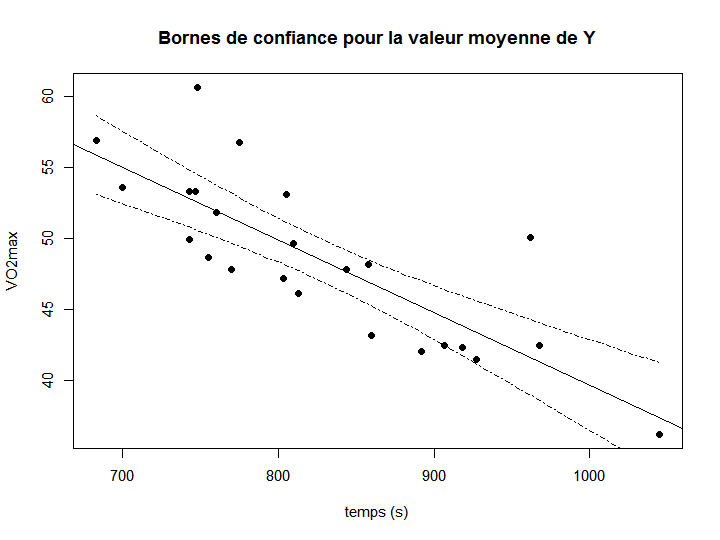
\includegraphics[width=9cm]{ICmoy.png}
\end{frame}

\begin{frame}[t]{Exemple  3 (suite)}

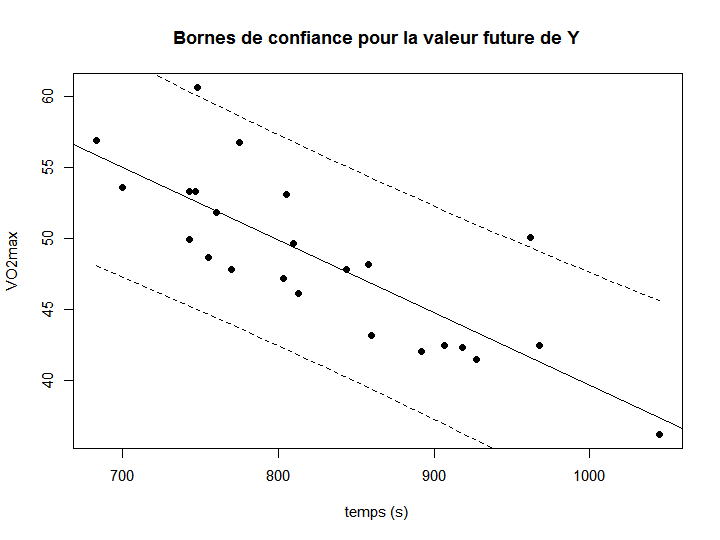
\includegraphics[width=9cm]{IPfutur.png}
\end{frame}




\section{Qualité de l'ajustement}

\subsection{Coefficient de corrélation échantillonnal $r$}

\begin{frame}[t]{Rappel de la corrélation}
On pourrait montrer que \alerter{$\beta_1=0\Leftrightarrow\rho=0$},\\ alors dans une relation linéaire, il n'y a corrélation que si la pente est différente de zéro.
\end{frame}

\begin{frame}[t]{Estimation  de $\rho$}

{\small
On a $\rho=\beta_1\dfrac{\sigma_X}{\sigma_Y}$, alors il y a un lien  entre les estimations de $\beta_1$ et  de $\rho$.

\medskip
$\rho$ est estimé par le coefficient de corrélation échantillonnal $r$ \\(lui aussi compris entre -1 et 1):
$$\hat\rho=\alerter{r=\hat\beta_1\dfrac{s_X}{s_Y}}=\frac{S_{XY}}{\sqrt{S_{XX}S_{YY}}}=\frac{\sum\limits_{i=1}^n(X_i-\overline{X})(Y_i-\overline{Y})}
{\sqrt{\sum\limits_{i=1}^n(X_i-\overline{X})^2\sum\limits_{i=1}^n(Y_i-\overline{Y})^2}}
.$$

\begin{tabular}{ccc}
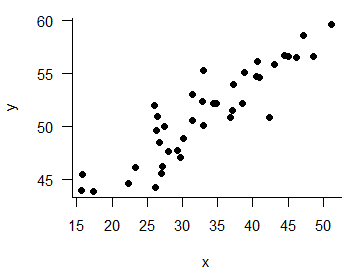
\includegraphics[width=3cm]{rho9.png}&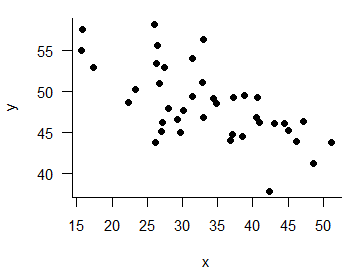
\includegraphics[width=3cm]{rho6.png}&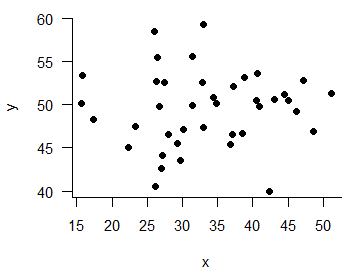
\includegraphics[width=3cm]{rho1.png}\\
 $\rho_{\text{simulé}}=0,9$ & $-0,6$ &$ 0,1$\\
$r =0,90$ & $-0,640$ & $0,041$\\
$R^2= 0,809$ &$0,409$&$ 0,0017$
\end{tabular}
}

\end{frame}


\subsection{Coefficient de détermination $R^2$}

\begin{frame}[t]{Le coefficient de détermination $R^2$}

Est-ce que $X$ "explique  bien" $Y$?

\medskip
Le \underline{coefficient de détermination} ($R^2$), soit \alerter{la proportion de
la variabilité dans les $Y_i$ qui est expliquée par le modèle de régression} (donc par $X$), est une quantité très utilisée pour juger de la qualité d'un modèle de régression linéaire.

\begin{align*}
R^2&=\frac{SS_R}{SS_T}\\
&{\color{gray}{=\frac{S^2_{XY}/S_{XX}}{S_{YY}}=\frac{S_{XY}}{S_{XX}}\frac{S_{XY}}{S_{YY}}}}\\
&{\color{gray}{=\hat{\beta}_1\frac{S_{XY}}{S_{YY}}=\hat{\beta}_1^2\frac{S_{XX}}{S_{YY}}}}\\
&=r^2.
\end{align*}

\end{frame}


\begin{frame}[t]{Exemple 4 sur le $VO_2max$}
%$\Rightarrow$ \alert{Plus la corrélation entre $X$ et $Y$ est forte, plus grande sera la proportion de la variabilité dans la valeur des $Y_i$ expliquée par le modèle de régression}.

Coefficient de détermination :

\vspace{3cm}

Coefficient de corrélation échantillonnal :
\end{frame}


\section[Valider postulats]{Validation du modèle: Analyse des résidus}


\begin{frame}[t]{Validation du modèle: Analyse des résidus}
La validité des conclusions de l'analyse statistique du modèle de régression
dépend du respect des postulats (P1) à (P4).

\small
\begin{itemize}
\item[P1] {\bf  linéarité:} l'espérance de $Y_i$ est linéaire en $X_i$;
\item[P2] {\bf homoscédasticité:} $V(E_i)=V(Y_i)=\sigma^2$  (ne dépend pas de $X_i$);
\item[P3]  {\bf indépendance:} $E_1,\ldots,E_n$ indépendants (idem pour $Y_i$);
\item[P4]  {\bf  normalité:} $E_i\sim$ loi normale autour de la droite.
\end{itemize}
\normalsize

\medskip
Comme ces \alerter{postulats portent tous sur le comportement aléatoire des termes d'erreur $E_i$}, nous les vérifierons à l'aide des résidus
$$
e_i=Y_i-(\hat{\beta}_0+\hat{\beta}_1X_i)=Y_i-\hat{Y}_i.
$$
\end{frame}


\subsection{(P1) Linéarité}

\begin{frame}[t]{(P1) Linéarité: Validation graphique}


\begin{itemize}
\item \alerter{Un graphique de dispersion des paires $(x_i,y_i)$}: devrait montrer un nuage de points distribués de façon symétrique autour d'une ligne droite.
\item \alerter{Un graphique des paires $(\hat{Y}_i,e_i)$}: devrait montrer un nuage de points distribués symétriquement autour de l'axe des abscisses.
\end{itemize}
\end{frame}

\begin{frame}[t]{Exemples de nuages de points}

\vspace*{-3mm}

{\small
\begin{tabular}{cc}
Linéarité raisonnable&Linéarité raisonnable\\
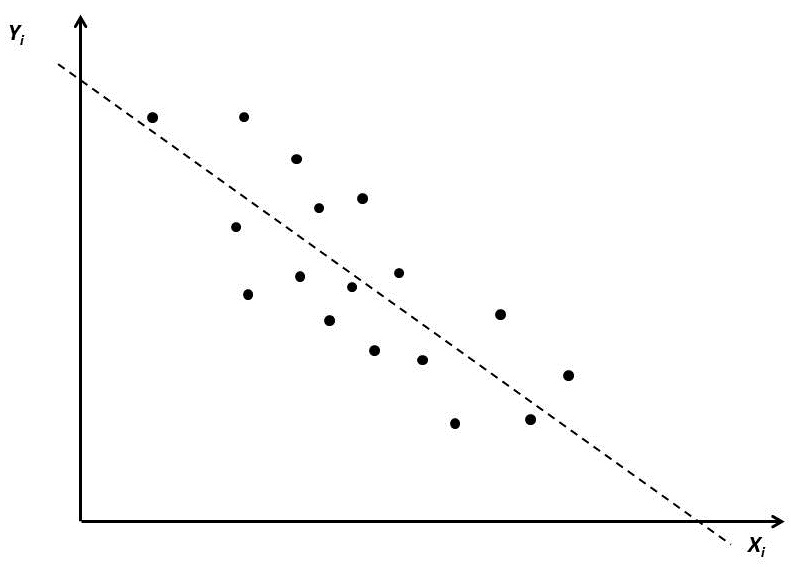
\includegraphics[width=1.8in]{yixiOK2.jpg} &
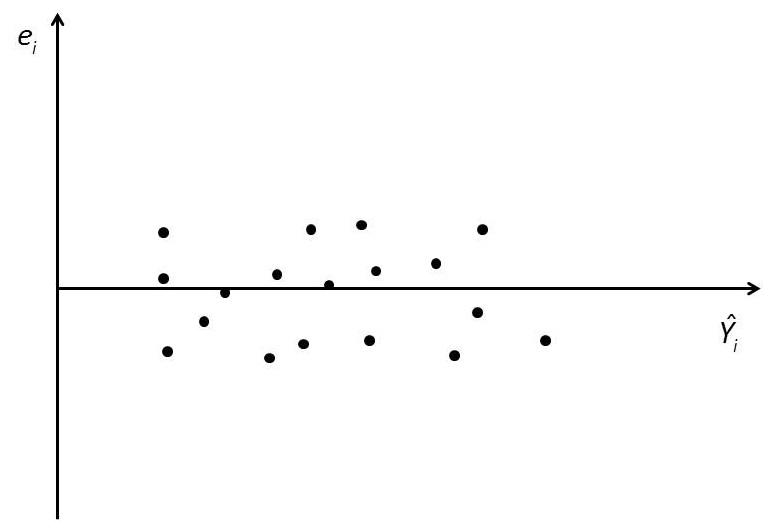
\includegraphics[width=1.8in]{eiyiOK2.jpg} \\
Linéarité déraisonnable&Linéarité déraisonnable\\
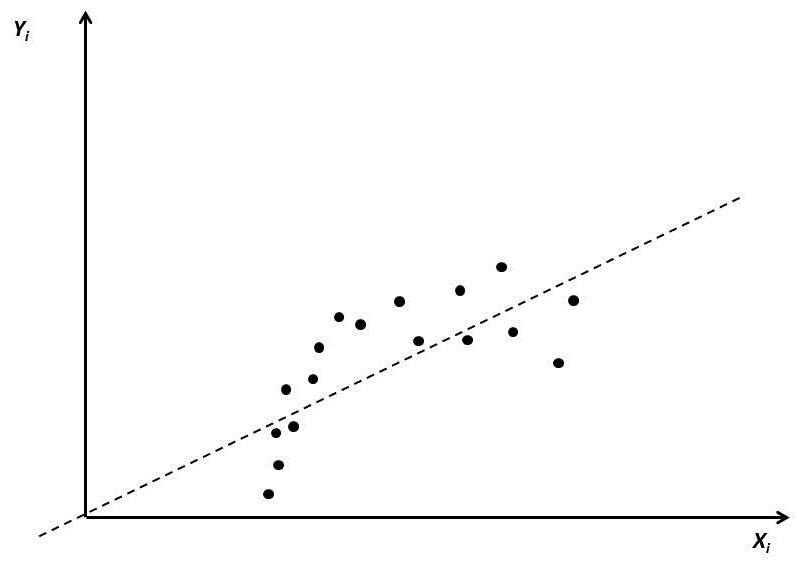
\includegraphics[width=1.8in]{yixiNOTOK2.jpg} &
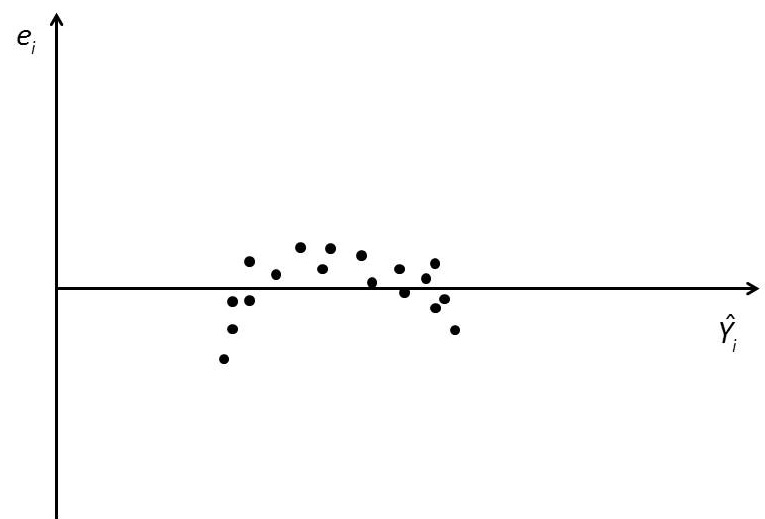
\includegraphics[width=1.8in]{eiyiNOTOK2.jpg} \\
\end{tabular}
}
\end{frame}

\subsection{(P2) Homoscédasticité (homogénéité de la variance)}

\begin{frame}[t]{(P2) Homoscédasticité}
\begin{itemize}
\item \alerter{Un graphique des $e_i$ en fonction des $\hat{Y}_i$}: devrait montrer que la variabilité des $e_i$ demeure constante pour toute valeur de $\hat{Y}_i$.
\end{itemize}
\end{frame}

\begin{frame}[t]{Exemples de nuages de points}

\vspace*{-3mm}

{\small
\begin{tabular}{cc}
Homoscédasticité raisonnable&\\
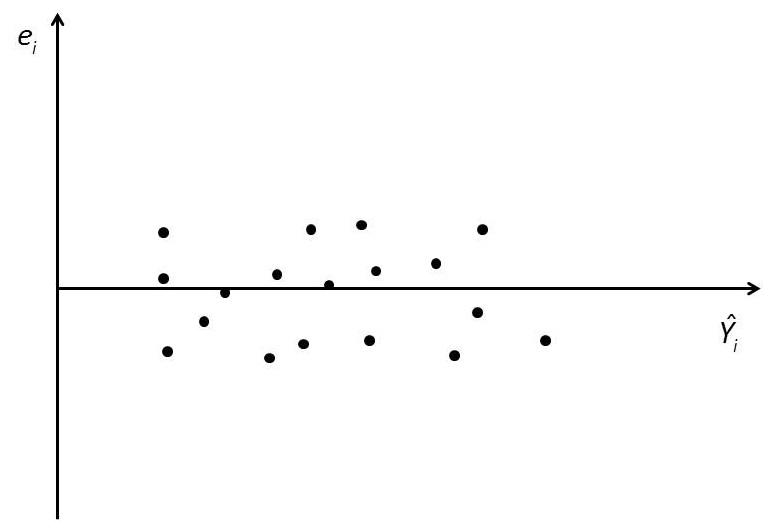
\includegraphics[width=1.8in]{eiyiOK2.jpg} &\\
Homoscédasticité déraisonnable&Homoscédasticité déraisonnable\\
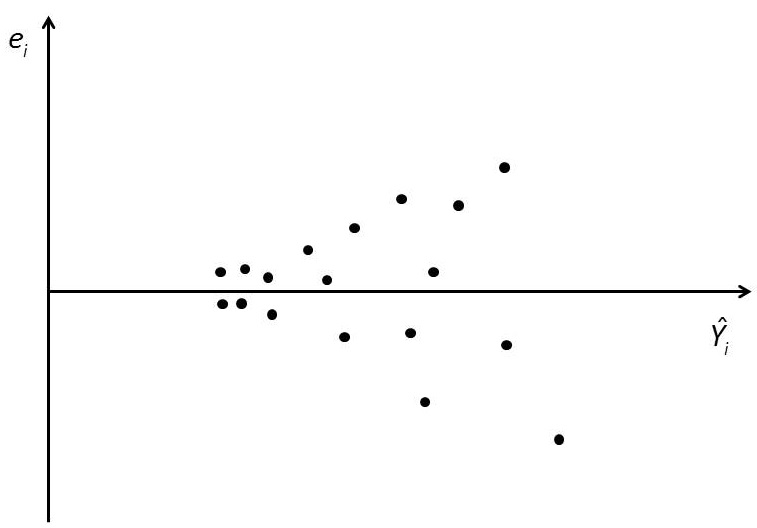
\includegraphics[width=1.8in]{hetero1-2.jpg} &
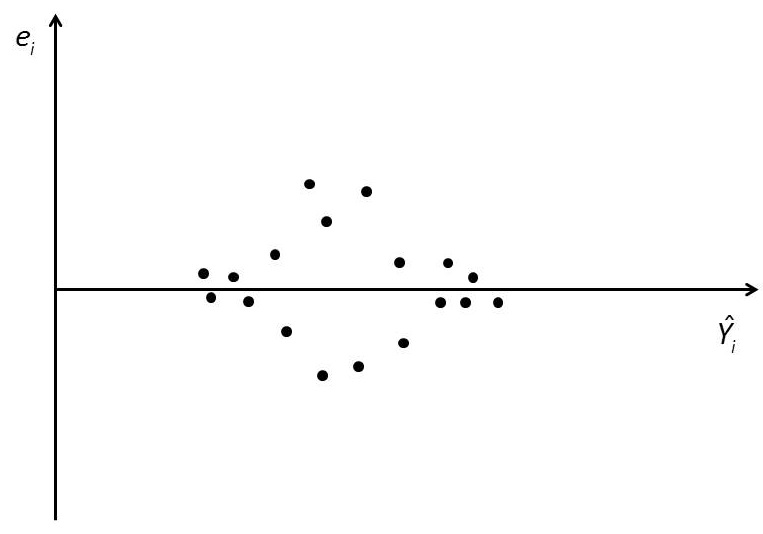
\includegraphics[width=1.8in]{hetero2-2.jpg} \\
\end{tabular}
}
\end{frame}



\subsection{(P3) Indépendance}

\begin{frame}[t]{(P3) Indépendance: Difficile à vérifier!}

{\small
C'est la collecte des données qui en est garante. Il faut s'assurer qu'\alerter{aucune variable à part $X_i$ n'ait pu avoir une influence sur les valeurs observées}.

\medskip
Exemple d'une mauvaise collecte:
\begin{itemize} \item les observations 1, 2, 3, 4 sont prises par l'employé A qui a tendance à surestimer $Y$;
\item les mesures 5, 6, 7 et 8 sont prises par l'employé B qui a tendance à sous-estimer $Y$;
\item Problème: les observations prises par un même employé seront corrélées.
\end{itemize}
}
\end{frame}

\begin{frame}[t]{Données chronologiques}

{\small
Il peut aussi y avoir de la corrélation lorsque les observations sont prises de façon trop rapprochées dans le temps (ou l'espace).\\
Si les valeurs de $i=1,\ldots,n$ correspondent à un \underline{ordre chronologique}, le \alerter{graphique des $e_i$ en fonction de $i$ } pourrait révéler un problème de corrélation positive entre les résidus rapprochés (``effet de grappe'').
}

\begin{center}
\begin{tabular}{cc}
Pas d'effet chronologique & Effet de grappe\\
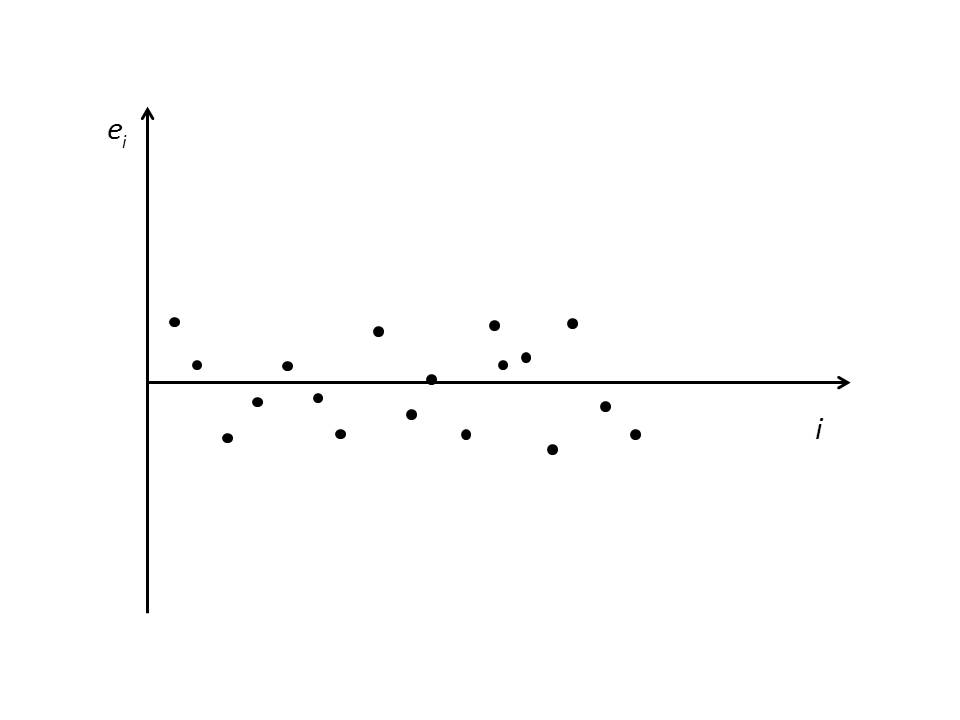
\includegraphics[width=2.17in]{eiiOK.jpg} &
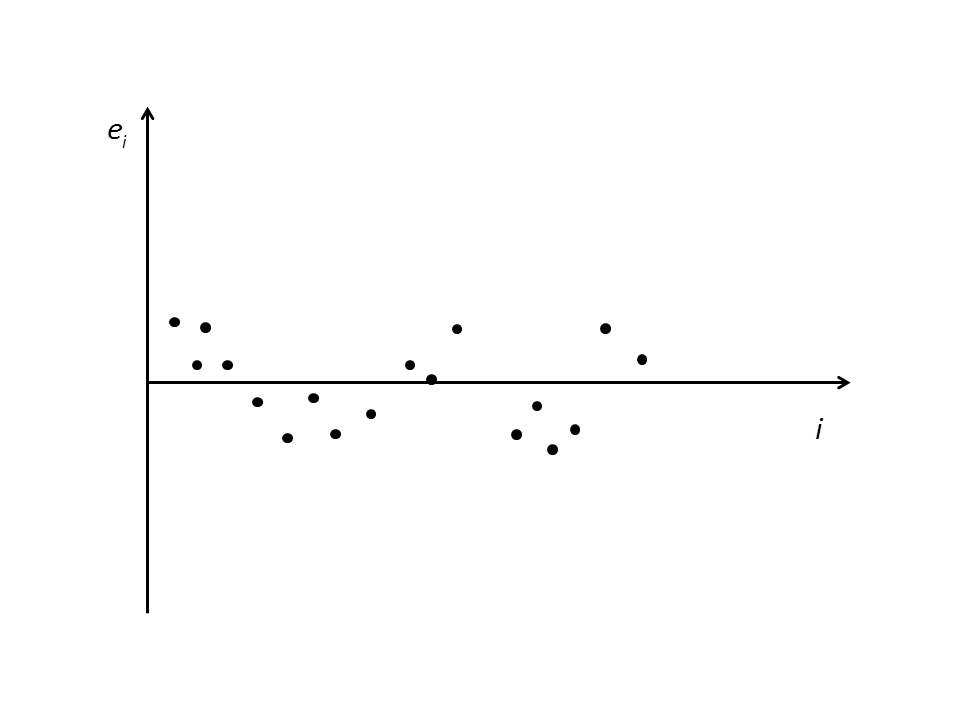
\includegraphics[width=2.17in]{eiiNOTOK.jpg} \\
\end{tabular}
\end{center}
\end{frame}


\subsection{(P4) Normalité}

\begin{frame}[t]{(P4) Normalité}
\begin{itemize}
\item \alerter{histogramme des résidus}
\item \alerter{graphique quantile-quantile normal des résidus }
\item \alerter{diagramme en boîte des résidus}
\end{itemize}
\end{frame}

\begin{frame}[t]{Exemple 5 sur l'absorption d'oxygène}
% Des graphiques permettant de valider les postulats d'homoscédasticité et de normalité pour l'exemple sur l'absorption de l'oxygène suggèrent que l'hypothèse d'homoscédasticité semble raisonnable, mais on peut mettre en doute la normalité ...
\vspace*{-3mm}

\begin{tabular}{ll}
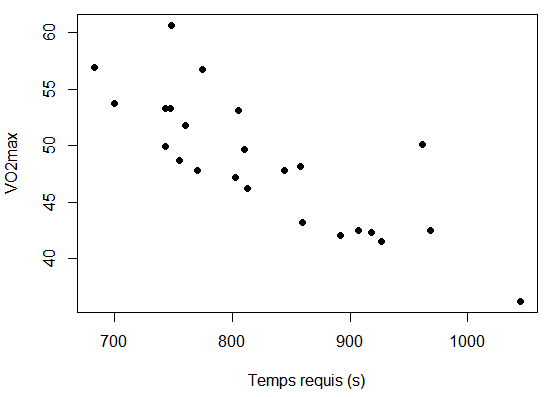
\includegraphics[width=1.8in]{Ex9_4-R1.png} &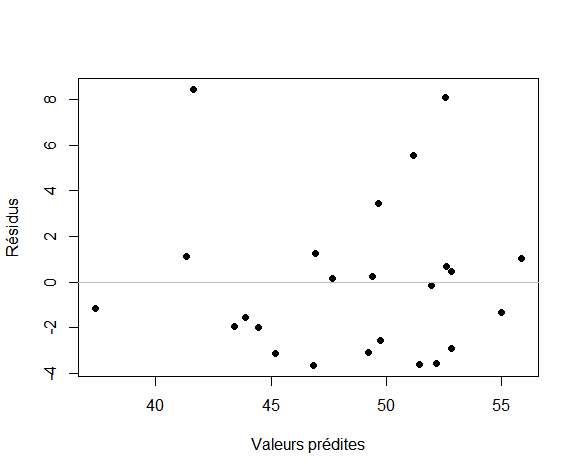
\includegraphics[width=1.8in]{Ex9_7-R1.png}\\
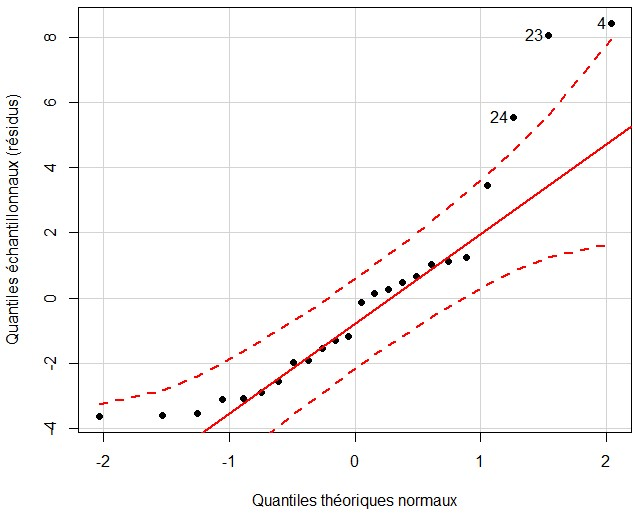
\includegraphics[width=1.8in]{Ex9_7-R3.jpg} & 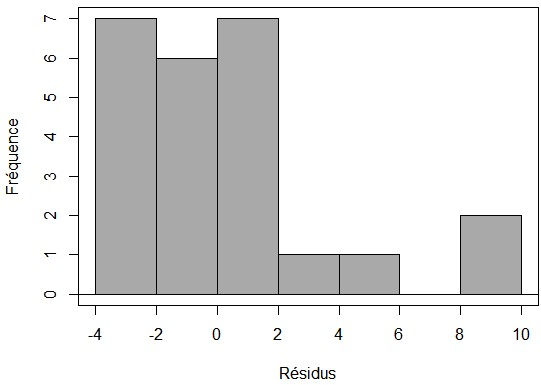
\includegraphics[width=1.8in]{Ex9_7-R2.jpg}
\end{tabular}
\end{frame}

\subsection{Solution aux problèmes: transformer $X$ et/ou $Y$}\label{sec:transfo}

\begin{frame}{Bibliographie}
 	Ce document est rédigé avec Beamer ainsi qu'une classe .cls fourni par Jérôme Soucy. Les diapositives sont adaptées des diapositives créées par Thierry Duchesne et Emmanuelle Reny-Nolin pour le cours STT-1900. Les graphiques proviennent de ces mêmes diapositives.
 	\printbibliography
 	\vfill
 	\footnotesize Pour signaler une erreur dans ce document, veuillez écrire à l'adresse :~\href{mailto:julien.miron@mat.ulaval.ca}{julien.miron@mat.ulaval.ca}.
 \end{frame}

\end{document}

